% REMEMBER: You must not plagiarise anything in your report. Be extremely careful.

\documentclass{l4proj}
%
% put any additional packages here
%

\begin{document}

%==============================================================================
%% METADATA
\title{Deep learning for analysing immune cell interactions}
\author{Leonore Papaloizos}
\date{\today}

\maketitle

%==============================================================================
%% ABSTRACT
\begin{abstract}
    Motivate; set aims; describe work; explain results.
    \vskip 0.5em
    ``XYZ is bad. This project investigated ABC to determine if it was better.
    ABC used XXX and YYY to implement ZZZ. This is particularly interesting as XXX and YYY have
    never been used together. It was found that
    ABC was 20\% better than XYZ, though it caused rabies in half of subjects.''
\end{abstract}

%==============================================================================

% EDUCATION REUSE CONSENT FORM
% If you consent to your project being shown to future students for educational purposes
% then insert your name and the date below to  sign the education use form that appears in the front of the document.
% You must explicitly give consent if you wish to do so.
% If you sign, your project may be included in the Hall of Fame if it scores particularly highly.
%
% Please note that you are under no obligation to sign
% this declaration, but doing so would help future students.
%
\def\consentname {Leonore Papaloizos} % your full name
\def\consentdate {\today} % the date you agree
%
\educationalconsent


%==============================================================================
\tableofcontents

%==============================================================================
%% Notes on formatting
%==============================================================================
% The first page, abstract and table of contents are numbered using Roman numerals and are not
% included in the page count.
%
% From now on pages are numbered
% using Arabic numerals. Therefore, immediately after the first call to \chapter we need the call
% \pagenumbering{arabic} and this should be called once only in the document.
%
% Do not alter the bibliography style.
%
% The first Chapter should then be on page 1. You are allowed 40 pages for a 40 credit project and 30 pages for a
% 20 credit report. This includes everything numbered in Arabic numerals (excluding front matter) up
% to but excluding the appendices and bibliography.
%
% You must not alter text size (it is currently 10pt) or alter margins or spacing.
%
%
%==================================================================================================================================
%
% IMPORTANT
% The chapter headings here are **suggestions**. You don't have to follow this model if
% it doesn't fit your project. Every project should have an introduction and conclusion,
% however.
%
%==================================================================================================================================
\chapter{Introduction}

% reset page numbering. Don't remove this!
\pagenumbering{arabic}

\section{Motivation}

Picture your immune system as a speed date. Your immune cells go on quick dates with other immune cells, who tell them about their life. The immune cells might be more or less under the influence of substances. The success of the discussion between the two immune cells during their speed date determines how your immune system is going to react as a whole. The consumption of substances might help make the reaction more positive, or might make a situation worse. Your immune system might be pleased with the date, and react positively, or an immune cell might get offended by their date, and trigger a negative response. % These dates could happen very fast with immune cells moving on to their next date, but could also be prolonged into longer relationships.

%The two partners we are studying are T cells and dendritic cells.
%long-term, non monogamous

% biological response
Formally put, the initiation of an immune response in our immune system depends on the interaction strength between different types of immune cells. Certain types of immune cells relay information about their environment to other types immune cells, who can then trigger an appropriate response depending on the what they have learned from the other cell about the environment. The environment might contain substances like foreign, dangerous bodies. These interactions between immune cells can be enhanced or inhibited by the application of drugs. Studying the reactions of immune cells under the influence different types of drugs is key in the development of drugs for diseases such as viral infections or auto-immune diseases.

\section{General problem and our idea}

One way of studying the interaction of immune cells is through microscopic images obtained in artificial settings. We can place immune cells in a dish and study them under a microscope under different experimental conditions, which could be different types of drugs being injected into the dish. Microscopic images of these cells can then be systematically captured.

We are however not interested in how these images are captured, but how they can be analysed. Microscopic images are often analysed with proprietary software which is costly to maintain and whose inner workings are hard to understand. On the other hand, applying deep learning techniques to biomedical data is becoming increasingly popular and more accessible, while obtaining promising results. The problem we are looking at is applying deep learning to the analysis of images of immune cells. We want to explore how deep learning could be used to systematically explore immune cell interaction from microscopic images. The aim is to assess whether using deep learning in the field of immunology can provide any useful information on interaction levels between immune cells under different experimental conditions.

%==================================================================================================================================
\chapter{Background}

\section{Immunology concepts}

\subsection{Our immune system} \label{bg:immunesystem}

Our immune system consists of organs, cells and groups of cells working in unison to defend us from outside organisms that could pose a danger to our health. Such outside forces could be harmful bacteria or parasites. The human body is a haven for these to thrive in, at our detriment. Our immune system protects us by attacking these foreign bodies – antigens – when they are detected and filed as dangerous. The key in this exchange is for our immune system to recognise which bodies are ours, and which are outsider, potentially dangerous forces (\cite{http://www.imgt.org/IMGTeducation/Tutorials/ImmuneSystem/UK/the_immune_system.pdf}).

\begin{figure}[h]
    \centering
    \begin{subfigure}[h!]{0.3\textwidth}
        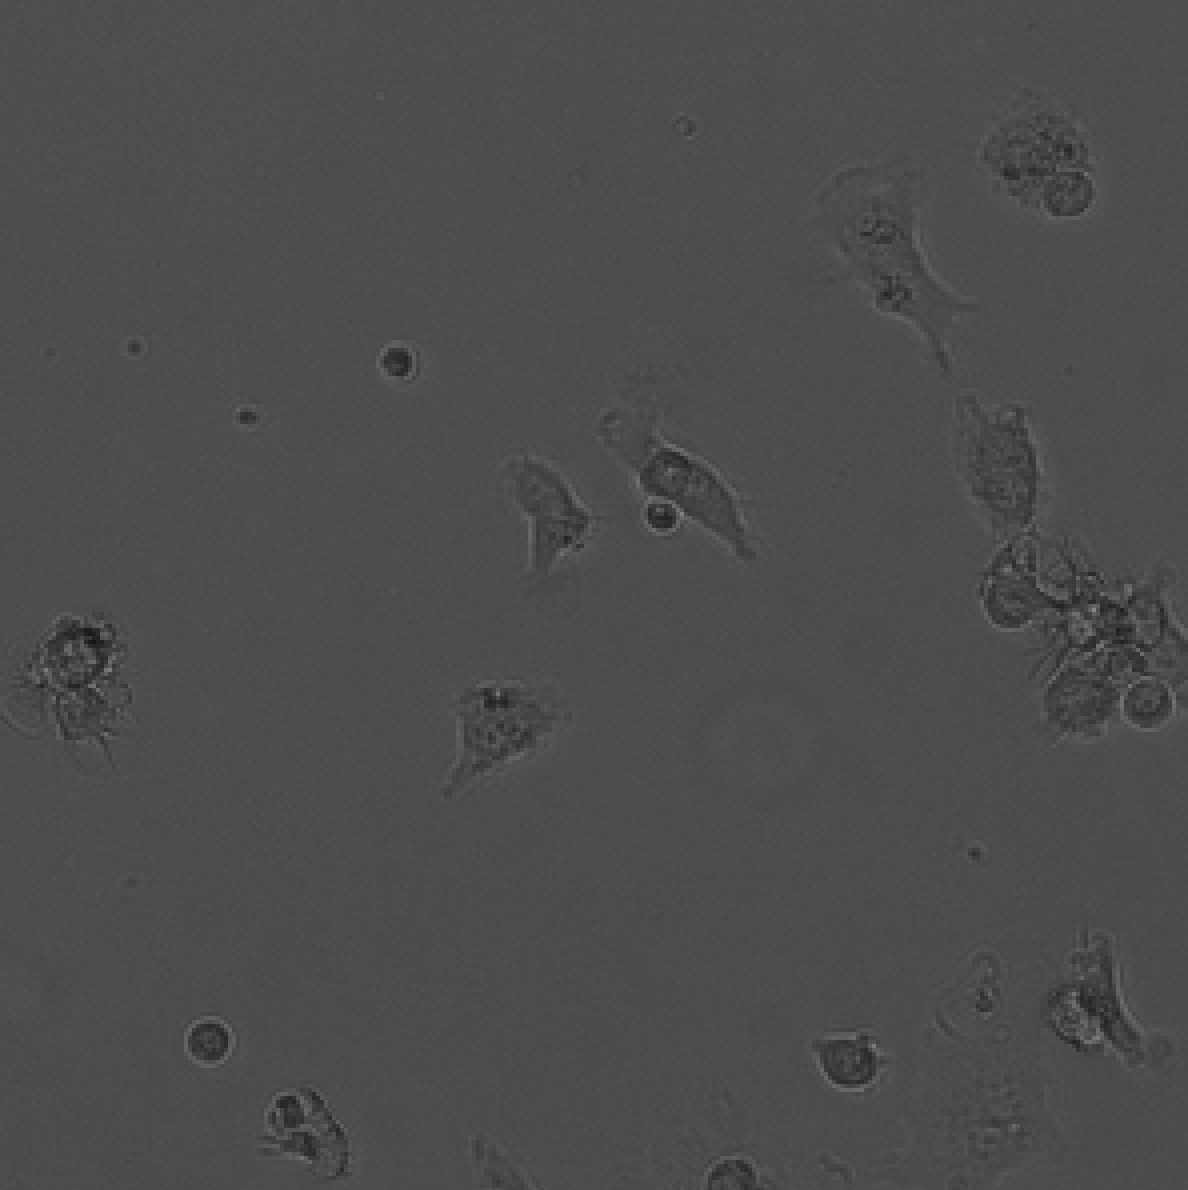
\includegraphics[width=\textwidth]{dissertation/figures/example_DCs.png}
    \end{subfigure}
    \begin{subfigure}[h!]{0.3\textwidth}
        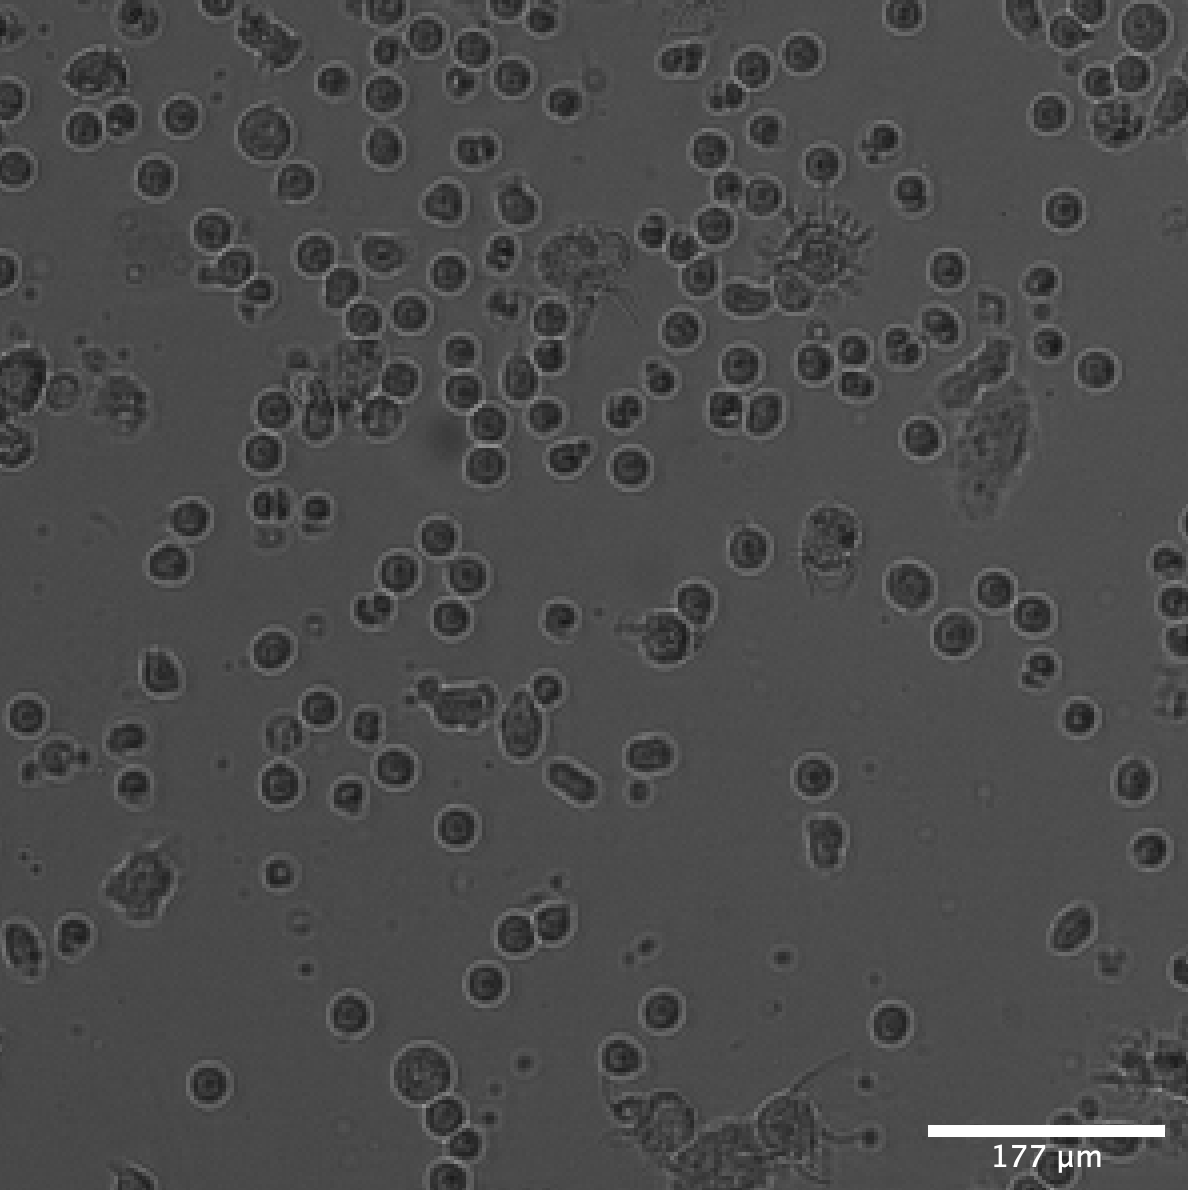
\includegraphics[width=\textwidth]{dissertation/figures/example_Tcells.png}
    \end{subfigure}
    \caption{Microscopic images of dendritic cells (left) and T cells (right) in an assay. Scale: , 200x zoom.}
\end{figure}

\begin{figure}[h]
    \centering
    \begin{subfigure}[h!]{0.3\textwidth}
        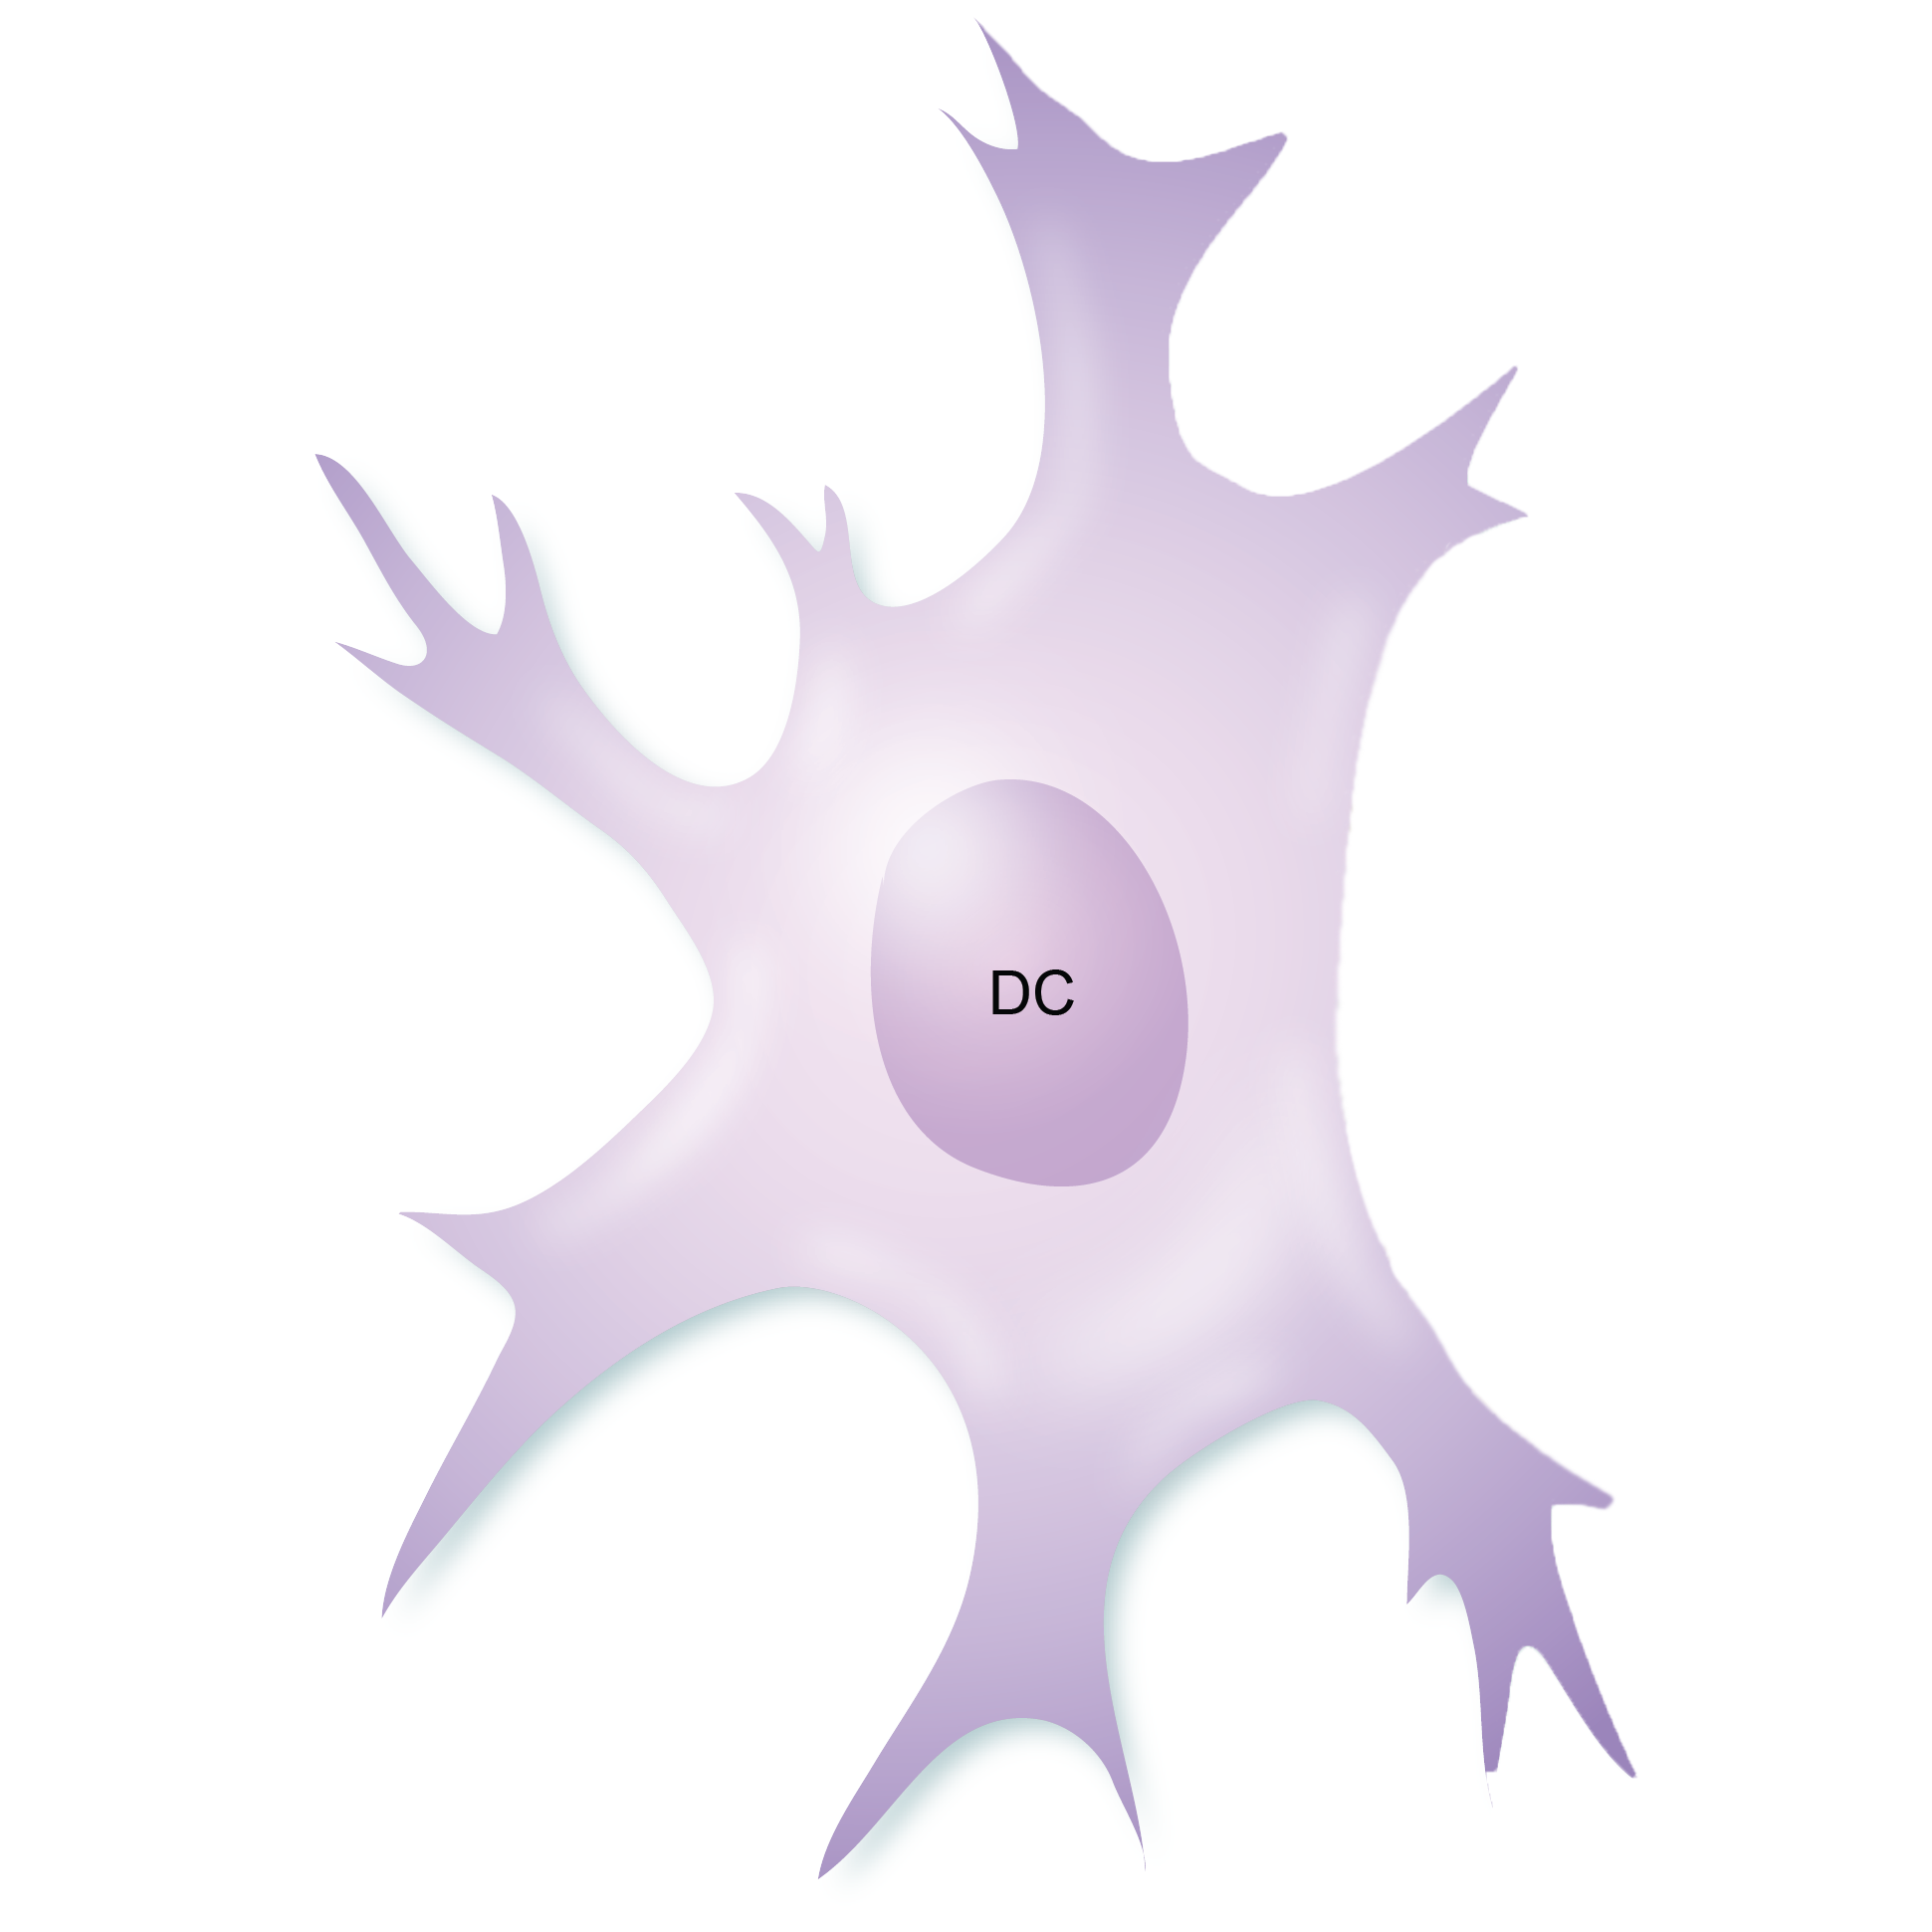
\includegraphics[width=\textwidth]{dissertation/figures/model_DC.png}
    \end{subfigure}
    \begin{subfigure}[h!]{0.3\textwidth}
        
\includegraphics[width=\textwidth]{dissertation/figures/model_Tcell.png}
    \end{subfigure}
    \caption{Model of a dendritic cell (left) and a T cell (right). Adapted from \cite{https://www.immunology.org/public-information/bitesized-immunology/systems-and-processes/t-cell-activation}}
    \label{eval:graphs}
\end{figure}

% What is the scale of the microscopic images?

The key defenders of our bodies are thus the actors of our immune systems. The actors we are interested in for the purpose of this research are T lymphocytes – "T cells" – and dendritic cells – DCs. Dendritic cells are "sentinels" and initiate our immune system's responses by processing their environment and sending the information over to T cells. T cells are "master controllers" and trigger the appropriate immune response, if any, from the information they have received from dendritic cells (\cite{https://www.immunology.org/public-information/bitesized-immunology/cells/dendritic-cells, https://www.youtube.com/watch?v=hRvyCYyab68}). [how to give more detail without losing reader? is this sufficient?]

%They interact with T cells, interactions which might be transient if nothing is to be triggered, or more communicative (\cite{https://www.youtube.com/watch?v=hRvyCYyab68}).

%The idea is that we can stimulate this interaction between dendritic cells and T cells through different drug components, both for inhibition or increase of level of interaction.

\subsection{Effects of interaction between immune cells} \label{bg:interaction}

Antigens, which is the encapsulating term for all threats to our immune system, can be fought by antibodies, which are defensive proteins produced by our immune system. More specifically, antibodies are produced by some immune cells in a process which starts in T cells, and in some cases is activated by T cells seeing antigens on the surface of dendritic cells (\cite{https://elifesciences.org/articles/06994}). Hence, the interaction between dendritic cells and T cells is critical in the decision for our immune system to produce agents to defend our body.

The purpose of this dissertation is to evaluate how much interaction is witnessed between immune cells. There is existing work in the field of immunology looking into the effects of these changes in interaction. Benson et al. show how the generation of antibodies might be impacted by T cell and dendritic cell interaction. They studied how dendritic cells and T cells interacted in mice's immune systems, both in terms of duration and whether or not interaction was indeed witnessed. This interaction was studied under different conditions, with different drug compounds being used to attempt to drive interaction or inhibit it. They found that in conditions where compounds were blocking interaction between T cells and DCs, less antibodies were generated, meaning that the mice were not defending themselves as much. Hence, the study of the impact of compounds on the interactions between immune cells can tell us how our immune system could react.

\subsection{Implications}

Concepts and research highlighted in Sections \ref{bg:immunesystem} and \ref{bg:interaction} show that changes in interactions between immune cells control the way in which our immune system protects itself. Hence, analysing the interaction between immune cells under different experimental conditions poses a particular interest in the field of immunology for studying immune responses. We want to analyse this interaction with the help of deep learning techniques.

% title: qualifying interaction
\section{Concepts of interest in Deep Learning}

The following sections collate selected research that show how deep learning techniques could be applied in our context of study.

\subsection{Convolutional Neural Networks for image feature extraction}

%A number of approaches already use deep neural networks for classification from textual genome sequences, particularly for cancer type detection (\cite{https://www.biorxiv.org/content/10.1101/612762v1}, \cite{https://www.nature.com/articles/s41598-019-53989-3}).
Convolutional operations in neural networks were first introduced by Fukushima at the start of the 1980s for pattern recognition. They were later popularised by LeCun as a method for object recognition, once back-propagation was put to use as a learning procedure for networks. LeCun applied his convolutional neural network to digit recognition and classification. Since then, convolutional operations in neural networks have proven to be successful to extract features from images. In a recent medical example, Shen et al. trained a convolutional neural network structure to detect breast cancer from mammography screenings and which showed competitive results compared to commercial systems (\cite{https://www.nature.com/articles/s41598-019-48995-4}).
[how much research to cite in this context? there is a lot available]

\subsection{Autoencoders for dimensionality reduction}

An autoencoder is a type of neural network trained to map its input to its output from a compressed representation of the input, as shown in Figure \ref{fig:autoencoder}. The compressed representation of the input obtained from the bottleneck layer is a \textit{coded} representation of the input, while the final output of the network is the \textit{decoded} version of the input. Autoencoders are not trained to learn a perfect copy of the input data, but a smaller, compressed copy with features which the neural network learns to be most important to be able to gain and overall understanding of the input. Autoencoders were first introduced in the 1980s (LeCun, DE Rumelhart) and are traditionally used for dimensionality reduction and feature extraction (\cite{http://www.deeplearningbook.org/contents/autoencoders.html}).

\begin{figure}[h!]
    \centering
    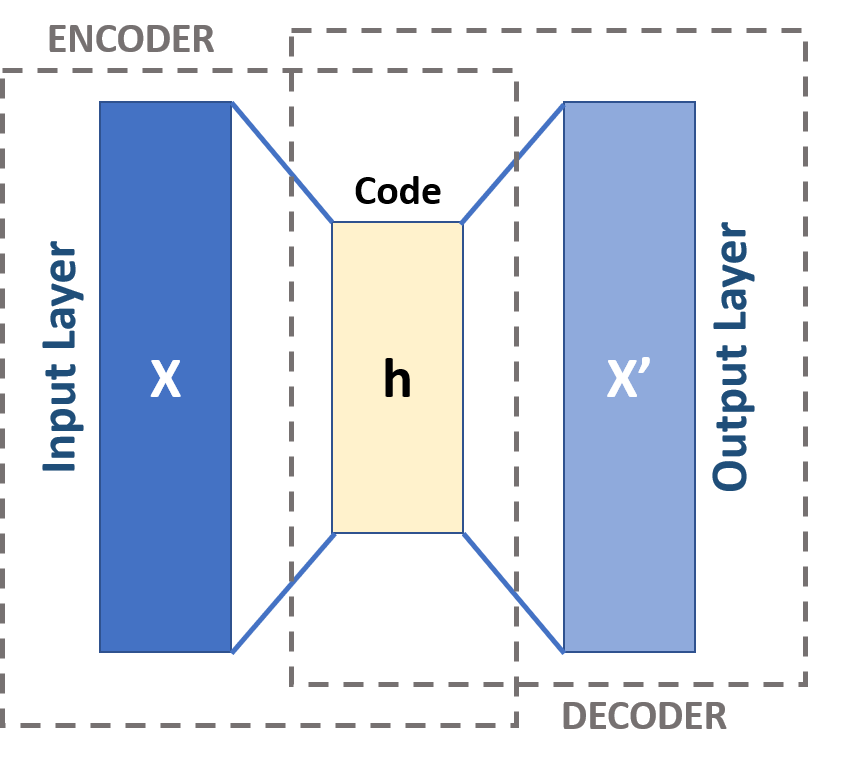
\includegraphics[width=0.45\textwidth]{dissertation/figures/autoencoder_schema.png}
    \caption{Autoencoder representation. To be recreated in Photoshop. Current source: Wikipedia}
    \label{fig:autoencoder}
\end{figure}

Zamparo and Zhang, 2015 (\cite{https://arxiv.org/pdf/1501.01348.pdf}) show that autoencoders can be successfully applied for dimensionality reduction in the context of biomedical data. Their autoencoder approach, applied to the unsupervised clustering of cell phenotypes, outperformed other dimensionality reduction techniques such as Principal Component Analysis (PCA). However, the context of this approach was not on imaging data.

% http://arxiv.org/abs/1809.00027
Nonetheless, autoencoders have been successfully used for reducing the dimensionality of large imaging data by using convolution operations in their structure. Saenz et al. successfully used convolutional autoencoders for feature extraction from climate imaging data. %More famously, convolutional autoencoders have been shown to be efficient in improving the clustering of the MNIST dataset, when visualised with high-visualising techniques like t-sne and UMAP. t-sne and UMAP are of interest to us as they allow to project high-dimensional data onto 2 dimensions (or three in the case UMAP). Using them allows us to assess whether or not our data has some underlying structure – e.g. whether or not we can cluster cells according to different experimental conditions.

\subsection{Deep regression models}

Deep neural networks can also be used to make real-valued prediction, rather than categorised. Moussavi-Khalkhali and Jamshidi used autoencoders trained with Stochastic Gradient Descent to predict timeseries data \cite{https://ieeexplore.ieee.org/document/7838202}.

\section{Finding structure in high-dimensional data}

The data we are studying consists of images of cells obtained through high content screening (HCS). HCS is a method for capturing images of cells in multi-well plates, using high-resolution microscopy \cite{https://www.ncbi.nlm.nih.gov/pubmed/23035272}. A plate captured with high content screening can yield a large number of images in very high-resolution, e.g. 2048x2048 pixels. This makes the analysis of the physical characteristics of a cell possible at a granular level. However, it could be of interest to us to gain an understanding of the overall structure of the data, in which case the high dimensionality of each data point (each image) will be harder.

The following sections highlight available techniques that can be used to look for structure in a group of high-dimensional data points.

%High content screening (HCS) is a method for capturing images of cells in multi-well plates, using high-resolution microscopy. It can be used to analyse physical characteristics of the cells captured on images. HCS is a choice method for analysing how compounds can alter cells from images, i.e. drug discovery \cite{https://www.ncbi.nlm.nih.gov/pubmed/23035272}.

\subsection{t-SNE}
t-distributed stochastic neighbor embedding (t-SNE) was developed in 2008 by van der Maaten and Hinton as a technique to map high-dimensional data to a two- or three-dimensional space. t-SNE can find structure in high-dimensional data points by using the local relationships between data points and optimising results using gradient descent. [how much detail to go into? don't want to go off tangent]%These local relationships are defined using a Gaussian probability distribution in high dimensional space, and then recreated using the Studnet t-distribution.

\subsection{UMAP}
Uniform Manifold Approximation and Projection for Dimension Reduction (UMAP) is a dimensionality reduction technique which was published in 2018 and has shown competitive results compared to t-SNE.

\section{The place of Deep Learning in immunology}

There is a number of existing research that use broader machine learning techniques in the field of immunology. Muh et al (\cite{https://www.ncbi.nlm.nih.gov/pubmed/19516900/} applied Support Vector Machines (SVMs) to the study of allerginicity. Allergic reactions are triggered when a immune system wrongly triggers an immune response and produces antibodies to attack a normally harmless substance, such as dust (\cite{https://www.immunology.org/policy-and-public-affairs/briefings-and-position-statements/allergy}). The SVMs were used to analyse the DNA sequences of known allergens and known non-allergens. The aim was to try and make accurate predictions on unseen sequences and classify them as either allergenic or non-allergenic. The model achieved 95.3\% accuracy. %Similarly, MP et al. \cite{https://www.ncbi.nlm.nih.gov/pubmed/20144194/} used a Bayesian classifier and a decision tree to predict the likelihood of degenerative disorders from the sequencing of antibodies.

[other example here]

\bigskip
This section has demonstrated that immunology-related fields such as cancer detection have successfully applied deep learning methods in their research to obtain promising results, and that immunology researchers have also successfully made use of machine learning techniques. [CONFIRM: Furthermore, deep learning has been applied in immunology for sequencing based analysis, (as well as cell segmentation?).] The research cited here highlights that there is an array of methods available to process high-dimensional, visual data and analyse it with the help of deep learning. However, there seems to be a lack of research into the qualitative and quantitative analysis of immune cell interactions from imaging data through these techniques. This paper will thus focus on filling this gap by using deep learning to extract features from images of cells in order to uncover qualitative or quantitative data about the interactions between types of immune cells. [INTRODUCTION?: Subsequently, the results of this research could show whether this shows promise and should be explored further in the future.]

%==================================================================================================================================
\chapter{Materials and Methods} \label{sec:mm}

This chapter covers the image materials that were available to analyse, how they were processed, and which methods were applied to them. The details of the implementation of these methods is then discussed in Section \ref{implementation}.

\section{Immune cells dataset}

\subsection{Setup}

The images that were used for the purpose of this research were provided by researchers in immunology at the University of Glasgow. The images were captured from multi-well plates with a commercial INCell Analyzer Machine (\cite{https://www.gelifesciences.com/en/us/shop/cell-imaging-and-analysis/high-content-analysis-systems/instruments/in-cell-analyzer-2500-hs-high-content-analysis-hca-imaging-system-p-04586}). As established in Section \ref{bg:immunesystem}, the type of immune cells we are studying are T-cells and dendritic cells (DCs). Each plate to be imaged in the INCell Analyzer Machine contains a grid of wells. Each well is assigned and label and experimental conditions. T-cells, dendritic cells, and compounds related to the experimental conditions are injected in the well. For distinction, the cells are loaded with fluorescent dyes: the T-cells are dyed with a green dye, and the dendritic cells are dyed with a red dye. After imaging, we obtain three field-of-view images per well:

\begin{itemize}
    \item a Brightfield image, which shows both T-cells and dendritic cells (Figure \ref{fig:brightfield})
    \item an image showing only the T-cells, which has been captured thanks to the fluorescent green dye (Figure \ref{fig:tcells})
    \item an image showing only the dendritic cells, which has been captured thanks to the fluorescent red dye (Figure \ref{fig:dcells}).
\end{itemize}

\begin{figure}[h]
    \centering
    \begin{subfigure}[h!]{0.3\textwidth}
        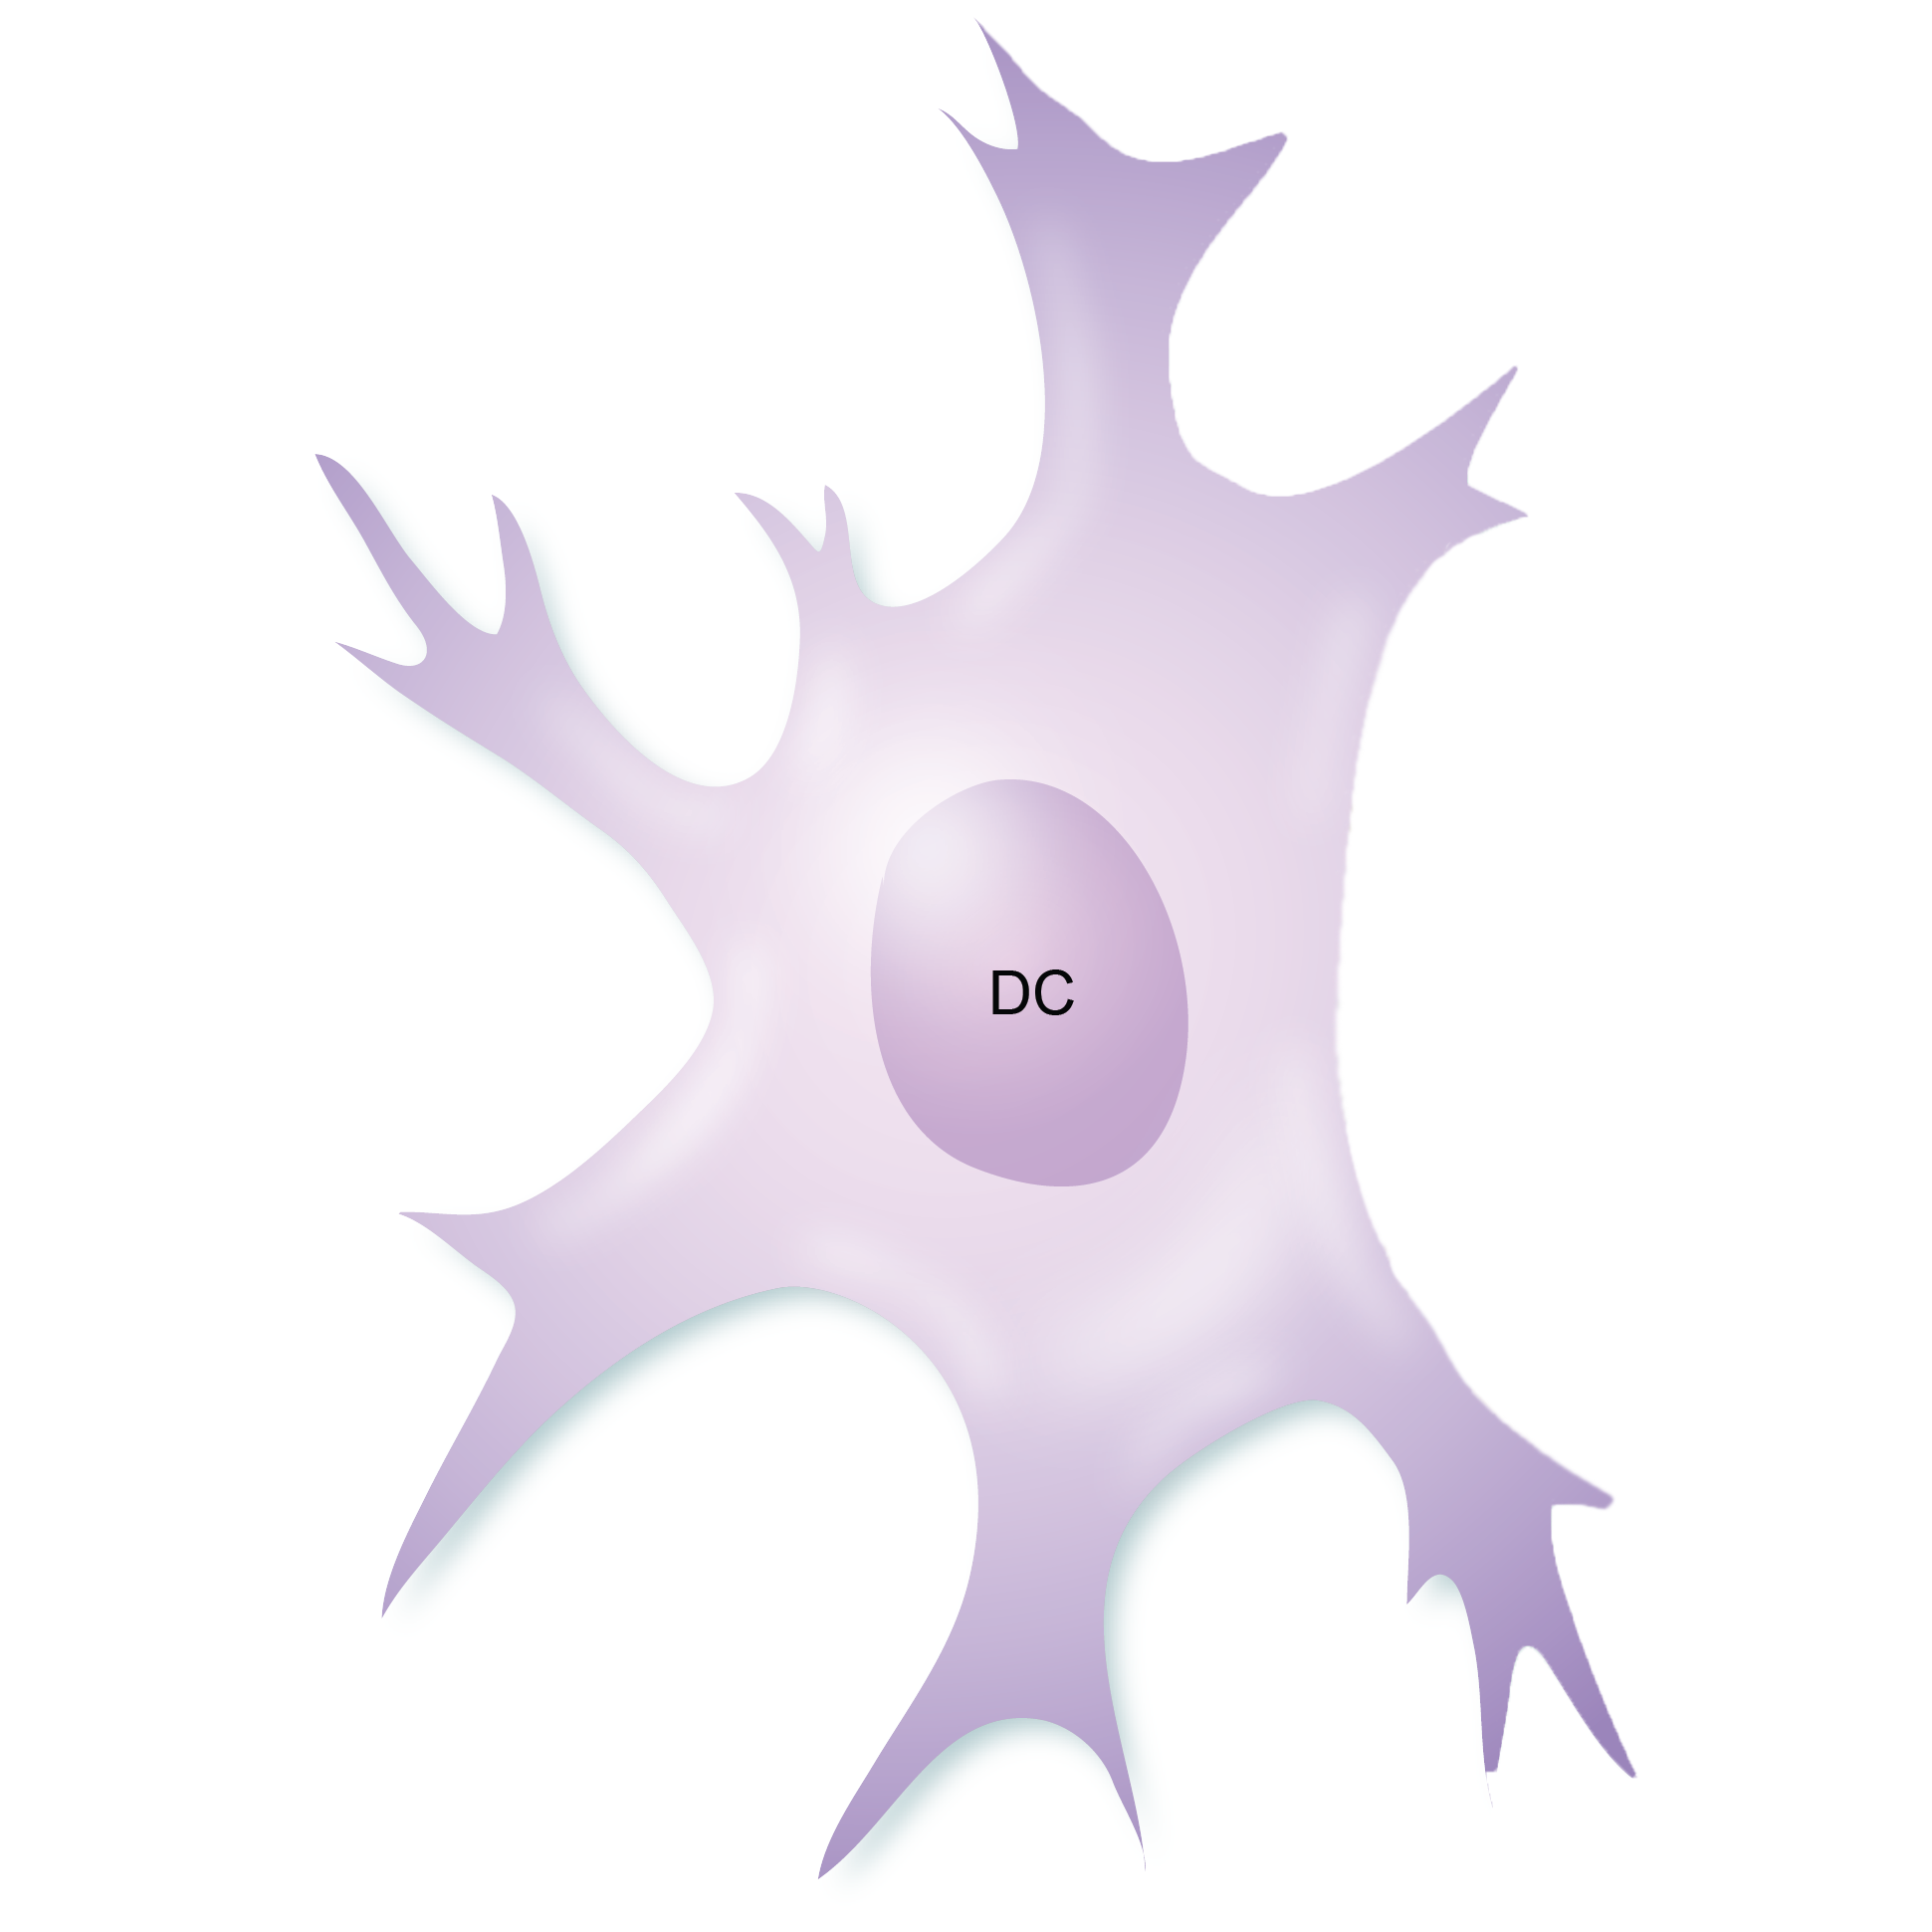
\includegraphics[width=\textwidth]{dissertation/figures/model_DC.png}
    \end{subfigure}
    \begin{subfigure}[h!]{0.3\textwidth}
        
\includegraphics[width=\textwidth]{dissertation/figures/model_Tcell.png}
    \end{subfigure}
    \begin{subfigure}[h!]{0.3\textwidth}
        
\includegraphics[width=\textwidth]{dissertation/figures/model_Tcell.png}
    \end{subfigure}
    \caption{Model of a dendritic cell (left) and a T cell (right). Adapted from \cite{https://www.immunology.org/public-information/bitesized-immunology/systems-and-processes/t-cell-activation}}
    \label{eval:graphs}
\end{figure}

\subsection{Picking images}

There was a large amount of images available from different well plates with different experimental conditions. However, each set of images represents about 8GB of data. Moving images about a file system and through disks or cloud filing system represented substantial time and was vulnerable to transfer errors. Hence, a limited number of plates were picked out for training and evaluation to make sure their consistency could be validated. The plates chosen had to be picked while keeping in mind the experimental conditions they represented, to make sure analysing them would yield something useful.

[TODO: explain in more detail if labels haven't been explained earlier on]
\begin{itemize}
    \item The ``DMSO" dataset: [TODO to be read over by Hannah] DMSO is a solvent that helps solubilise the drug compounds in a well as most compounds are not initially water soluble. The drug compounds being more soluble, they should then be able to have more of an impact.
    \item The ``balanced” dataset: this dataset contains an equal number of images in the three categories of stimulation: no drug simulation, stimulation with OVA peptide, and stimulation with ConA. This is to fight issues of class imbalance when training the model.
    \item The simpler dataset, with two categories: this  dataset contains an equal number of images in two categories: no drug simulation, and simulation with OVA peptide. This was picked in the hope that if no results are obtained with 3 categories, a model might be able to perform better with two.
\end{itemize}

\subsection{Preprocessing}
The datasets obtained from this setup consisted of 2048x2048 12-bit images in a 16-bit TIFF file. As mentioned above, each ``image” really consists of a set of three field-of-view images: the t-cells, the dendritic cells, and the Brightfield image. The Brightfield images were used to gain an overview of what the image might look like, but were discarded and not used for analysis.

%Fiji (ImageJ) was used to explore the images as the particular 12-bit format of the image in a TIFF file meant that standard image previewers reproduced the image as all black. Fiji also offered useful tools for testing image pre-processing methods, such as binary filters, thresholding, and background correction.

\bigskip
Each of the images sized about 8MB, and represented 4,194,304 pixels. Each plate had about 400 setups, which corresponds to 800 images when counting both the t-cell image and the dendritic cell images. This represented an issue of very high dimensions to deal with, and little images to feed into any kind of model.

\bigskip
Moreover, initial tryouts of reconstructing images with an autoencoder showed that it struggled with such small details. Figure () shows that even to the naked eye, the small white dots could easily be confused for dust on the screen.

\bigskip
[example figure]

\bigskip
The first idea was to make the images more palatable by a neural network by cutting up a set square subsection of the image. However, this still created an issue of limited input to the dataset. This was improved by passing a sliding window over the image, creating a hundred 192x192 images per file. This quickly expanded the size of the dataset, making it as big as 58000 samples in some cases. Smaller images also made more sense to the naked eye, hence it was assumed that a trained model would perform better with this gridded dataset.

\bigskip
For each subimage, it was then normalised with min-max normalisation to get a [0,1] range of values. From analysing the images, it was also found that a lot of background noise was in the pixel range of [0, 255] before normalisation, so before normalisation values below 255 were clipped.

\subsection{Outlier detection and labelling}

The provided images sometimes contained some noise, coming from issues such as water droplets in the wells. These outlier images were detected because their pixel values seemed to always be between 0 and 255. Instead of removing them from the dataset entirely, it was decided to keep them in to see if a model could make sense of them as a category. These were labelled as "Faulty".

All the images came with an Excel sheet giving information about the plate layout. Each image was given a letter and a name, and the Excel sheet gave information about drug stimulation, compound ID number, or compound concentration. These Excel sheets were not automatically parsable as types of drugs or location in the sheet might vary from one to the next, hence labelling had to be hardcoded and handchecked.

\subsection{Combining images to visualise interaction}
\bigskip

For feeding into a model, the gridded, processed images had to be combined for them to make sense for the task of analysing interaction. For one set of microscopic image in one condition, the t-cell black and white image and the dendritic cell black and white image were combined in an RGB image where the red channel corresponded to the dendritic cell, the green channel corresponded to the t-cell, and the blue channel was left blank.

Figure () illustrates how the processed and combined sub-image might look, for each of the different categories we are trying to look at in this task.

[row of three images here]

\section{Image segmentation}

Image segmentation refers to the process of separating out different parts of interest of an image for different purposes. The purpose of image segmentation applied to this dataset of immune cells was both to attempt to correct any noisy background from the supplied images as well as use image segmentation to obtain numerical data about cells in the images.

\subsection{Background correction}

A common issue for microscopic images obtained systemically through different screening systems is that of a noisy background [ref]. This can usually be corrected through different methods, such as flat field correction or the rolling ball algorithm [ref]. Flat field correction takes a ``neutral” image without anything (i.e. cells) added to it to later use it as a reference image to perform background correction on any other images. However, the provided dataset did not come with a flat field image. As such, alternatives had to be explored.

\bigskip
All the images in the original, uncombined dataset are black and white, with the details of interest (the cells) in bright white spots. However there might be some gray details in the image that the naked eye cannot see immediately, but that could influence how a machine learns. Hence we need a method that will separate out the cell pixels from the background. We can do this by obtaining a binary mask of the image. The white pixels will correspond to the cells, and the dark cells will be the background. We can remove the background of the original image by multiplying it with the mask. Only the cells will remain in the image.

\subsection{Analysing interaction}

By using the above described method, we also obtain a binary mask of the image. This binary mask can be used for further calculations. A common metric for evaluating image segmentation quality is intersection over union [ref]. In our case, we can use this metric to calculate an area of overlap between the two separate images for a t-cell and a dendritic cell, corresponding to the same experimental condition. We can use the concept of overlap to quantify the level of interaction between cells. This number could then be used attached to an image as an input to a regression model in order to evaluate whether we can try a model to recognise a value of interaction from an image.

\section{Autoencoders}

[TODO: this might be covered in background a bit]
Autoencoders are a particular type of neural network that have a symmetrical layer structured around an encoded representation. The aim of an autoencoder is to map an input to its output as close as possible while reducing its dimensions. The hope is that if an image is reduced to a certain number of dimensions, and a neural network is able to reconstruct the original image very closely just based on that compressed representation, then that compressed bottleneck representation of the image should be a good enough, reduced input we can then feed into other models.

\bigskip
[autoencoder figure here]

\subsection{Visualising high dimensional data}

One use for autoencoders and their capacity to reduce dimensions is that it could help the performance of high-dimensional visualisation techniques. High dimensionality visualisation techniques such as t-sne and UMAP can help visualise if there is an inherent structure to the data. This can be used in the context of analysing immune cell interactions by observing whether or not different clusters are found, and whether or not they correspond to different drug conditions. In this case, we would be able to differentiate different levels of interaction from the images.

\subsection{Regression}

We can also use the encoding part of the autoencoder to build a regression model and evaluate whether the model is capable of predicting interaction values from an image.


%==================================================================================================================================

\chapter{Implementation}

\section{System diagram}

Figure \ref{fig:system} can help the reader to gain understanding how each of the materials and methods used as described in Section \ref{sec:mm} fit together.

\begin{figure}[h!]
    \centering
    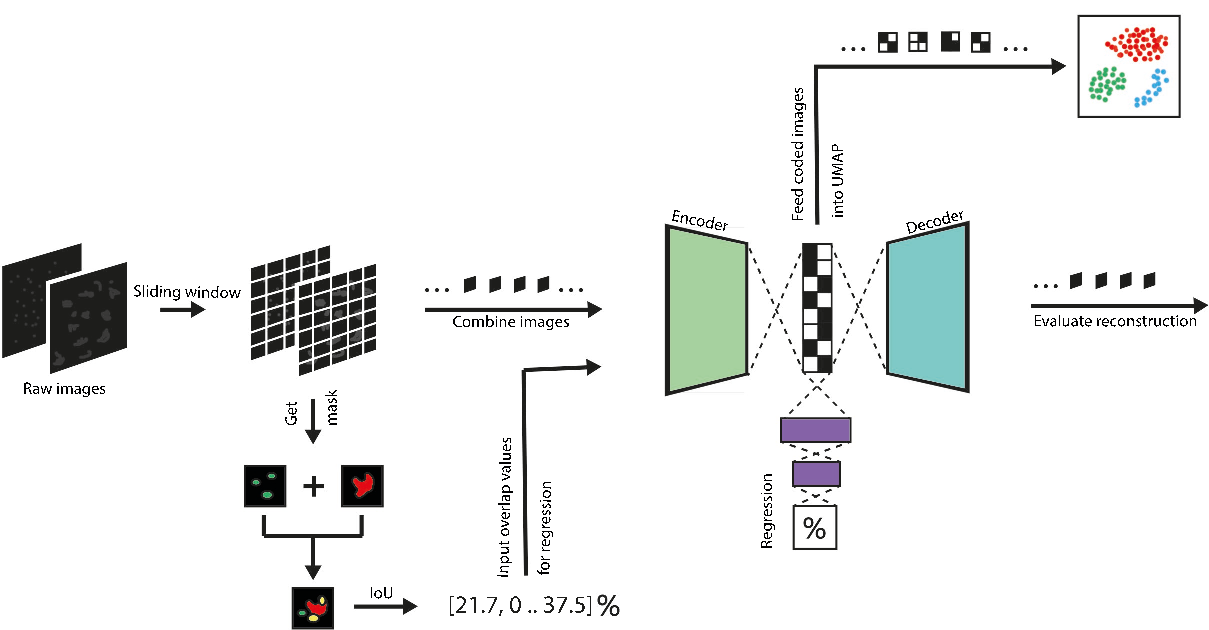
\includegraphics[width=\textwidth]{dissertation/images/system_diagram.jpg}
    \caption{[TODO on Photoshop] System diagram showing how each image will be decomposed and analysed.}
    \label{fig:system}
\end{figure}

\section{Pre-processing}

Firstly, before feeding them as input into any model, the images of cells had to be pre-processed. This is already partly discussed in Section \ref{}. This section will go over some specifics and justify some choices that were made.

\bigskip
The following list provides a step-by-step of the process:
\begin{enumerate}
    \item For each dataset, all the images of T cells and dendritic cells were picked out. Their corresponding filenames were retrieved.
    \item The filenames were sorted to keep images from the same well next to each other in memory.
    \item Each image was partitioned into sub-images through a sliding window approach. The window was of size 192x192 and yielded a 100 same-sized images. The original image was 2048x2048 so the right and bottom borders of the image were discarded.
    \item Once this gridded dataset was obtained, each T cell image was combined in a RGB image with its dendritic cell counterpart, stored in index i and index i+100 respectively.
    \item For each combined image, noise was removed through low value pixel clipping. Min-max normalisation was then applied to put all images in the same [0,1] range.
\end{enumerate}

Some choices made in the above have to be justified.

\subsection{Sliding window}

The sub-image window size was chosen to be 192 because of the pooling and upsampling operations in autoencoders. When an image is processed in the encoder part of the autoencoder, and the 2x2 pooling operations are applied, the image dimensions are reduced by a factor of 2. Each pooling operation has a corresponding upsampling operation in the decoder part of the autoencoder. If a pooling operation results in a decimal dimension, the number is rounded up. The corresponding upsampling operation would then double that number, which would result in a different dimension in the output of the autoencoder. Hence, we had to pick a size that would be big enough to show enough cells, but we also had to pick a size which meant the image could be divided by 2 for a large amount of times, depending on the number of hidden layers. To illustrate, if we apply a division by to the number 200 three times, the image can be upsampled and reconstructed correctly, however if it is reduced 4 times, then after the 4th operation we obtain a 13x13 image and the first upsampling operation creates a 26x26 image. A size which is a multiple of 8 bypasses that issue for a larger number of operations. A 192x192 image can be reduced 6 times, when it reaches dimensions of 3x3, without running into upsampling issues.

\subsection{Image combination}

Images of each type of cells on their own would not make much sense on their own when the aim is to quantify the level of interaction. Hence they have to be combined. The advantage that the provided dataset has is that it comes with the T cells and the dendritic cells separated by means of fluorescent dyes, hence no image segmentation technique had to be used to be able to separate the image out into the different types of cells and colour them in. Instead, each of the T cell and its corresponding DC, which were associated to the same file, were combined together in an RGB image, with the blue channel set to 0. The images were not combined in an absolute difference operation as we would have lost information of where the images overlapped i.e. interacted, which is what we are looking into in this research.

\section{Quantifying immune cell interaction}

To obtain the interaction measure from the images, multiple methods were tried out. Structural Similarity Index was computed, however because the images were so similar in general i.e. white blobs spread across a black background, the results were extremely similar across all cells in different experiment conditions (show image?). The idea was instead to obtain masks of the images and compute the intersection over union area as the interaction value. As the cells were bright blobs on a black background, and we did not have the task of separating T cells from dendritic cells, it was hoped that this would be straightforward. Both K-means and thresholding methods yielded good results.

\subsection{K-means}
K-means has been shown to perform well on colour segmentation. It was easy to initialise. OpenCV's K-means was used over sklearn's because over 1000 images, it performed a lot faster. [recompute] K-means was applied to the images with K=2 and 10 iterations for performance. First, K-means centers were initialised randomly. However, during training and validation it was found that this method of initialisation was yielding highly different results for the intersection over union metric at every run. Hence, some speed was traded for consistency and the kmeans++ center initialisation method was picked instead.

\subsection{Thresholding}
The alternative to K-means is thresholding. Thresholding depends on pixel value analysis. Usually, thresholding works well for images which have peaks of pixel values in their distribution. However, this was not the case for our images. First, the threshold value picked was the mean pixel value. This yielded acceptable results, however some noisy pixels still came through the mask.

[illustrate as you write !!!]

To fix that problem, the threshold value was set as the sum of the mean pixel value and the standard deviation. This decision was made on the hypothesis that the noise level of an image with a flat structure can be estimated from its variation.

\subsection{Image masks for background correction}
As mentioned in materials & methods, the images might have noise. Particularly in biomedical data, there has been research on background correction. Rather than fixing the background, we can evaluate whether removing the background entirely helps in this case by evaluating both masked an unmasked images.

\section{Convolutional autoencoder}

The main tool to be developed to exploit this dataset was a convolutional autoencoder. The autoencoder was built for two purposes: obtaining a smaller "code" representing each of the images to be fed into high-dimensional visualisation algorithms, and to be the starting block for a deep regression model.

\subsection{Structure}

The autoencoder was built using Keras \footnote{https://keras.io} for Python. We based our architecture off the standard Convolution --> Activation --> Pooling sequence of operations commonly used in convolutional neural networks (ref). The aim was to maximise the reduction of dimensionality while maintaining a satisfactory reconstructed image. Hence, the choice of number of hidden layers had to be made as a compromise.

The autoencoder was tuned by evaluation on a training and validation dataset. Its structure was established through both literature review and trial and error. The choice of hidden layer activation is PReLU, because of its evidenced benefit in improved loss (ref), as well as showing slightly better results in training. Moreover, convolutional layer sizes were kept quite high, instead making the neural network deeper to reduce dimension. Strides are used in the last layer instead of max pooling (why?) because results were slightly better. The choice of feature maps being higher in earlier layers comes from the encoded representation being smaller this way, as well as differences with the reversed being marginal. Finally, the output layer activation is sigmoid, as we are trying to predict a value between 0 and 1, as the images have been normalised.

\subsection{Deep regression}

The regression model was built on the encoder layers of the autoencoder. The structure of the regression layers of the model was kept simple. Only two fully connected layers are used, with a Dropout layer in between. Dropout has shown to make models more robust and prevent overfitting.
Both softplus and linear activations were tried for the regression model. The linear activation was accompanied with a kernel restriction on the keras model of non-negativity, as interaction cannot be negative. Softplus keeps its output values positive. The results were similar, however the linear function performed overall better.

%==================================================================================================================================
\chapter{Evaluation}

\section{Train-test dataset split}

A large amount of data was available to us. In order to best evaluate the performance of our trained autoencoder and regression models, part of the data was picked for training, and the rest was left out for testing. Part of the training data was used while training for validation and model checkpoints.

As explained in Section \ref{}, three datasets were picked out for research. Training was done on the balanced dataset. The balanced dataset was not prone to class imbalance issues, and contained an equal mix of images from each class: unstimulated immune cells, immune cells stimulated with OVA, and immune cells stimulated with ConA.

Part of this balanced dataset was kept untouched for testing. Two other datasets were used for testing: the DMSO dataset, and the two-category dataset.

The two-category dataset had two purposes: evaluating if the model performed better with differentiating between two classes instead of 3. Moreover the two-category dataset contained both labels of drug stimulation and drug concentration. It was hypothesised that maybe we could gather more information of interaction based on drug concentration rather than type of drug.

The DMSO dataset had issues because it was built from the balanced and two-category dataset and parts of the DMSO images were possibly used to train the balanced dataset. However, DMSO represents the conditions in which difference in interaction should be most visibile, thus it was still valuable to evaluate for results. However, it is considered "tainted".


%\section{Autoencoder}
%\subsection{Reconstruction}
%\subsection{2D Visualisation with t-sne and UMAP}
%\subsubsection{Matplotlib tool for outlier exploration}

%==================================================================================================================================
\chapter{Conclusion}

%==================================================================================================================================
%
%
%==================================================================================================================================
%  APPENDICES

\begin{appendices}

\chapter{Appendices}

\end{appendices}

%==================================================================================================================================
%   BIBLIOGRAPHY

% The bibliography style is abbrvnat
% The bibliography always appears last, after the appendices.

\bibliographystyle{abbrvnat}

\bibliography{l4proj}

\end{document}
